% % \documentclass[manuscript.tex]{subfiles}
% \documentclass[12pt,a4paper]{report} %,openright,twoside
% \usepackage{thesisstyle}
% \addbibresource{bib/PhD.bib}
% % \setcounter{chapter}{2}
% \begin{document}

\title{Super-resolution of Aeromagnetic Survey Data}
\author[1*]{Luke Thomas Smith}
\author[1]{Tom Horrocks}
\author[1]{Eun-Jung Holden}
\author[1]{Daniel Wedge}
\author[2]{Naveed Akhtar}
\affil{Centre for Data-Driven Geoscience, School of Earth Sciences, The University of Western Australia (M006), 35 Stirling Highway, 6009 Perth, Australia}
\affil{Department of Computer Science and Software Engineering, The University of Western Australia (M002), 35 Stirling Highway, 6009 Perth, Australia}
\date{\today}
% \maketitle{}

\begin{abstract}
    Contemporary super-resolution is a deep learning technique to increase the resolution and high-frequency details of raster data.
    However, despite the widespread success of super-resolution upscaling of natural photographs, its application to low-resolution geophysical surveys remains to be fully investigated.
    Previous applications to geophysical survey data generate training data pairs of low- and high-resolution grids by downsampling the high-resolution grid with standard image filters, which is a poor approximation to real-world low-resolution aeromagnetic grids constructed from sparsely sampled survey data.
    Moreover, the structural variation within the survey data depends entirely on the geological domain which is surveyed.
    This paper proposes an approach to super-resolution of aeromagnetic survey data using transfer learning from synthetic data that represents a wide range of realistic geological domains, to imrpove the generalisability of the resulting model.
    The approach uses realistic high-resolution and low-resolution pairs of gridded survey data, obtained by simulating aeromagnetic surveys of the data at close and wide line spacings.
    Structural accuracy of the method is improved using a secondary fine-tuning stage incorporating real-world survey data.
    The Local Texture Estimator neural network architecture was used, and qualitative and quantitative measures of the super-resolution performance are reported.
    The results demonstrate that the proposed method is capable of transforming regional scale aeromagnetic surveys to high-resolution for a wide range of geological features.
\end{abstract}

\section{Introduction}
We propose a method for super-resolution (SR) upscaling of aeromagnetic geophysics data from diverse geological provenance.
This method uses transfer learning \parencite{tanSurveyDeepTransfer2018} from magnetic data forward modelled from a collection of synthetic geological models with varied histories \parencite{jessellNoddyverseMassiveData2022}, and fine tuning with real-world data.
SR employed in this work leverages a contemporary neural network \parencite{leeLocalTextureEstimator2022}, with a realistic method for sampling high-resolution grids and gridding them to low-resolution.
The method is suitable for typical low-resolution regional aeromagnetic surveys in Australia.

\subsection{Resolution in geophysical data}
\label{sec:resinsurveys}
In exploration geophysics, the Earth's naturally occurring magnetic or gravitational potential fields can be used to survey the petrophysical expression of underlying geology.
These can be interpreted to inform geological mapping, resource modelling, and enhance the understanding of the subsurface.
Depending on the scale of investigation, surveys may be carried out from ground or airborne sensors.
Detailed ground-based surveys can be sampled at point spacings of tens of metres while avoiding local obstacles, but at a regional scale, aircraft are used to provide rapid and uniform coverage regardless of access constraints.
These airborne surveys collect data at wide line spacing to minimise cost, with lines in Western Australian low-resolution regional surveys typically \qty{400}{\m} apart, however, open access high-resolution surveys with line spacings of \qty{100}{\m} or closer are increasingly common.
Sampling along line is typically performed at \qty{10}{\Hz} or faster, which corresponds to several metres between samples at a nominal flight speed of \qty{70}{\m\per\s} \parencite{goodwinAirborneMagneticRadiometric2023}.
Because the power of shorter wavelengths in potential fields diminish with increasing distances from the source, aeromagnetic flights are flown as low as safety and topography permits.
Despite the use of precise navigation systems and skilled operators, these data are not collected in perfectly uniform lines at constant height, and the samples also contain noise components.

The subsequent analysis of surveyed potential fields generally relies on gridded data, and transforming irregularly distributed survey data to a regularised grids is the task of gridding.
There are several classes of gridding methods available.
Minimum Curvature gridding \parencite{briggsMachineContouringUsing1974} is routinely applied in industry applications, as it gives well characterised results in rapid time, with minimal manual intervention.
A comprehensive review of alternative spatial interpolation methods is presented by \textcite{liReviewComparativeStudies2011}.
Each method of gridding has characteristic interpolation traits (which when undesired are termed artefacts), but irrespective of the gridding process the detail resolvable in the output grid is a product of the sample height, sampling density, and the final cell size at which the grids are rendered.
Gridding at a finer cell size preserves higher frequencies present in the sampled data, resulting in greater detail.
This resolvable detail is termed resolution, and high-resolution details better define structures apparent in the data which are contextually important to interpretation.
When the cell size covers a quantified distance, the smallest resolvable detail can be expressed in terms of wavelength.
This is the grid's Nyquist wavelength, and is equal to twice the gridded cell size.
This corresponds to the widely known Nyquist frequency, i.e.\ the limit at which bandwidth-limited signals may be incorrectly resolved due to sampling below the Nyquist frequency, at half the sampling frequency.
For example, a potential field which lacks significant wavelength components shorter than \qty{200}{\m} will be adequately resolved by a grid with a cell size of \qty{100}{\m}, without spurious features known as aliasing.
Extending this concept, arbitrarily shrinking the cell size will not resolve additional detail unless also predicting features with wavelengths shorter than those present in the sample data.
These are limited by the sample spacing during acquisition.
% Low-resolution aeromagnetic survey data are the result of wide line spacings during acquisition, with the resulting grid cells predominantly being those predicted by interpolation between sparse sample points.
Achieving higher resolution traditionally requires additional sampling to increase the grid resolution. %, which refines structures in the response and reduces blocky textures and other gridding artefacts.
In addition to human interpretation, machine processing of geophysical data is benefitted by using higher resolution data, with the negligible cost of increased computational load.

A small number of regions in Western Australia are covered by high-resolution aeromagnetic surveys with a line spacing of 100 m or closer, and these are biased toward prospective geological terranes \parencite{howardAirborneGeophysicalCoverage2004}.
Therefore, example-based learning methods trained using these aeromagnetic data will be biased for performance in these domains, while lacking in those that have been so far regarded as unprospective.
Addressing costly data acquisition, common in geoscience \parencite{dawsonImpactDatasetSize2023}, can be done by transfer learning.
This assists example-based methods by using a larger source dataset which shares properties with the target dataset.
In order to improve the generalisation of an example-based neural network for regions without high-resolution coverage, we propose transfer learning \parencite{tanSurveyDeepTransfer2018} by first training a baseline model trained with synthetic data containing a broad set of geological domains, which is then fine-tuned with high-resolution survey grid data.
The synthetic geophysical data \parencite{jessellNoddyverseMassiveData2022} are forward modelled from 3D petrographic voxel models with varied geological histories.
These provide a diverse set of features, but these lack truly realistic characteristics, such as high frequency near surface magnetisation, and features from complex geological processes such as metasomatism or remnant magnetisation.

Thus, the approach made in this study to address the challenges of training an example-based model with limited suitable geophysical data is to make use of geologically diverse synthetic data, with a realistic sampling and gridding method to generate low-resolution data for training.

\subsection{Prior work}
Numerically, image interpolation can be done using interpolating functions, such as splines \parencite{keysCubicConvolutionInterpolation1981}, kriging \parencite{hansenInterpretiveGriddingAnisotropic1993} or other methods.
These methods are limited in their performance by the quality of their neighbouring observed values, and their distance.
Deep learning methods similarly use their spatial neighbours, but do so in the context of trainable filters, and across larger extents of the input.
In this way, deep learning super-resolution models are supported by latent information retained from the training dataset, in addition to information contained within the input being upscaled.

Instead of increasing the sampling density, the detail in potential field grids can be enhanced by calculating the potential as if it were sampled at a smaller source-sensor distance, in a process known as downward continuation \parencite{bullardDeterminationMassesNecessary1948}.
At large source-sensor distances, high frequencies are diminished below the noise floor to the point of unobservability, resulting in grids that show only broad scale features, typically representing spatially extensive features deep in the crust.
It is common for noise in the sampled grid product to be significantly increased in the downward continued product, limiting the useful vertical extent of the method to six times the cell size \parencite{dampneyEquivalentSourceTechnique1969,zuoDownwardContinuationTransformation2020}.
Downward continuation can be performed with field- or source-based methods \parencite{pilkingtonPotentialFieldContinuation2017}.
Resolution enhancement through neural network approaches to downward continuation \parencite{liStableDownwardContinuation2023,yeHighprecisionDownwardContinuation2022} is a promising research direction in super-resolution geophysics, but is distinct from the proposed line-spacing based method due to its use of paired vertically continued training data.

Recently, aeromagnetic resolution enhancement has been performed with deep learning SR \parencite{bavandsavadkoohiHighresolutionAeromagneticMap2023,smithMagneticGridResolution2022}.
Both methods operate on regional aeromagnetic data at four times scale, using variants of the SRGAN convolutional neural network originally by \textcite{ledigPhotorealisticSingleImage2017}.
The method of \textcite{smithMagneticGridResolution2022} demonstated SR methods are capable of upsampling low-resolution magnetic textures and predicting accurate short wavelengths for these data.
Comparison was made compared with numerical filters such as the bicubic filter.
However, the low-resolution data were created using a polynomial filter that suppressed high frequencies, rather than a real-world low-resolution geophysical sampling process.
The method of \textcite{bavandsavadkoohiHighresolutionAeromagneticMap2023} uses low- and high-resolution aeromagnetic data from regional surveys, with a realistic low-resolution transform from line spacing and sample altitude differences.
The dataset contains \qty{267} sample grids from surveys in Quebec, Canada, prepared from surveys with a low-resolution line spacing of \qty{800}{\m}.
The proposed method is distinct from these prior works with its use of extensive and geologically varied synthetic data in coordination with real survey data to improve generalisation for regional aeromagnetics in Australia, and the use of a modern MLP-based SR network.

Deep learning techniques for SR typically use paired high- and low-resolution image data, with the objective to learn the transform from low resolution to high.
This is an ill posed challenge, because many high-resolution images share the same low-resolution representation \parencite{dongImageSuperresolutionUsing2016}.
For photographs and natural image rasters with large representative training corpuses available, such as ImageNet \parencite{dengImageNetLargescaleHierarchical2009} and DIV2K \parencite{agustssonNTIRE2017Challenge2017}, SR methods have progressed to the point that high quality enhancement at four times scale is readily accessible to end-users \parencite[e.g.][]{wangRealESRGANTrainingRealWorld2021}.
Contemporary work with low-resolution transforms for natural images \parencite[reviewed in][]{moserHitchhikerGuideSuperResolution2023} has well characterised the research space and expected performance for upscaling photographs and digital images.
Prior work specific to this study are reviewed in \Cref{sec:2nnsr}.

Photographs and other natural images of interest to computer vision are typically created by capturing light from an image sensor or are explicitly mapped on a grid using a raster graphics program.
In these rasters, each pixel is regularly distributed, and the resolution is isotropic and a factor of the pixel density of the sampling sensor or the software defined grid.
These data are encoded to regular arrays of pixel values, commonly as three-channel rasters representing the red, green, and blue intensities of each pixel.
For natural images, a common approach to generating low-resolution data is to interpolate the high-resolution image to a smaller size using a transform such as bicubic downsampling.
Aerogeophysical grids are distinct from these image rasters due to the potential field sampling and grid interpolation process outlined in \Cref{sec:resinsurveys}, and the extent to which widely spaced low-resolution geophysical line data can be enhanced, and characteristics of the resulting super-resolved grids remain to be fully explored.
Most critically, aeromagnetic data are highly sampled in the direction of flight lines but are under-sampled in the line-perpendicular direction.
The resulting grid rasters may have isotropic cell size, but the frequency content in each axis is anisotropic, being a factor of the sampling frequency in the line-perpendicular (low) and line-parallel (high) directions.
Being sampled as a single component of the vector potential field, these data contain a single channel, and the data contain multiple sources of noise components.
Furthermore, the features present in these data are dependent on the subsurface geology, varying between smooth domains without significant near-surface magnetisation, through to highly deformed igneous stratigraphic units with complex high-intensity structures.
The recorded intensity values have high dynamic range, spanning tens of thousands of nanotesla, while contextually important features may be defined by tens of nanotesla \parencite{kovesiPhasePreservingTone2012}.
Because of these differences, pre-existing super-resolution models trained on large image corpuses are not suitable for predicting higher frequency signals in geophysical grids.

We propose a method that simulates the line sampling of both synthetic and real data, thereby more closely reflecting real-world low-resolution aeromagnetic data, at scales typical of those in exploration in Australia.

\subsection{Neural network super-resolution}
\label{sec:2nnsr}
Deep learning super-resolution (SR) is the task of predicting interpolating values to resolve rasters with a higher resolution, and has been predominantly performed in the domain of Convolutional Neural Networks (CNN) following the success of SRCNN \parencite{dongLearningDeepConvolutional2014}.
Recently, multi-layer perceptrons (MLPs) have become a state-of-the-art alternative for SR\@.
In an MLP (also known as a fully connected network), all neurons in a given layer are connected to all neurons in the immediately adjacent layers.
This contrasts with CNNs, where spatially related neurons are sparsely connected between layers via a convolutional kernel.
Fully connected MLP networks have been described for several decades, however, networks partly or entirely comprising fully connected layers saw little interest for SR following the success of SRCNN \parencite{dongLearningDeepConvolutional2014}.
It was noted in \parencite{arjovskyWassersteinGAN2017} that MLP networks were known to be a poor backbone in generative adversarial networks, an architecture which was seeing wide application in contemporaneous computer vision tasks.
One early SR network featuring fully connected layers was for multi-frame video super-resolution \parencite{chengFastVideoSuperresolution2012}, while another was used to investigate depth images \parencite{chenSingleDepthImage2018}.
\Textcite{tanFeatureSuperResolutionMake2018} aimed to create high-resolution feature maps for machine interpretation rather than subsequent visual observation.
Among the first image SR networks incorporating an MLP for human perception was by \parencite{tangDeepResidualNetworks2020}, who replace convolution operations in their network's final image reconstruction with a fully connected layer.
They suggest a fully connected layer outperforms convolutions for image reconstruction due to the wider receptive field of the MLP\@.

Implicit functions aim to learn a specific function parameterised entirely by the weights of a neural network.
In an image or geophysical grid context, the function may map grid coordinates to the value at those coordinates.
While extensively developed for point cloud and other 3D data \parencite[e.g.][]{jiangLocalImplicitGrid2020} there have been numerous examples for super-resolution.
These include SIREN \parencite{sitzmann2019siren}, LIIF \parencite{chenLearningContinuousImage2021}, and LTE \parencite{leeLocalTextureEstimator2022}.
Notably in these networks, the learnt function has continuous domain, despite the discretised grid input.
Super-resolution can be achieved by sampling the learnt function at any arbitrary grid cell size smaller than the original input \parencite{chenLearningContinuousImage2021}.
While a stand-alone MLP such as SIREN is capable of parameterising a single function, when used in an autoencoder framework (such as with LIIF or LTE), an arbitrary input can be encoded, upscaled, and subsequently reconstructed using fully connected layers \Cref{fig:ltenet}.
An autoencoder approach generalises MLP based super-resolution to any image or grid not seen in the training set.

Local texture estimator (LTE) \parencite{leeLocalTextureEstimator2022} is implemented in this work for its higher performance in the task of image super-resolution.
The encoder in LTE can use the feature extraction capability of traditional SR CNNs such as EDSR \parencite{limEnhancedDeepResidual2017} or RDN \parencite{zhangResidualDenseNetwork2018}, or a SwinIR \parencite{liangSwinIRImageRestoration2021} transformer-based encoder.
In the original implementation of the CNN SR networks, the extracted image features are upsampled and returned to the image domain by convolutional layers.
In LTE, the latent extracted features are further processed by the LTE network component before reconstruction to image space by an MLP\@.
An overview of the structure of the LTE network is shown in \Cref{fig:ltenet}.
Specifics of the LTE implementation to investigate the performance of SR for geophysical grids from a range of geological domains are detailed in \Cref{sec:2lte}.

\begin{figure}[hbtp]
    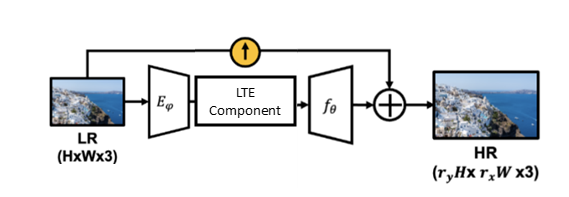
\includegraphics[width=\linewidth]{fig/p2/temp_lte.png}
    \caption[The LTE network]{
        A simplified representation of the super-resolution LTE network.
        The encoder is marked as \(E_\phi{}\).
        \(f_\Theta{}\) is an MLP network used as the decoder for image reconstruction.
        A long-range skip connection with simple upscaling is marked with an arrow.
        The LTE network block performs high-resolution upscaling of extracted features in the Frequency domain.
        Simplified from \textcite{leeLocalTextureEstimator2022}.
    }
    \label{fig:ltenet}
\end{figure}

The remainder of this paper is structured as follows.
\Cref{sec:2methods} describes the experimental design to generate low-resolution aeromagnetic survey grids from synthetic and real-world data, where \Cref{sec:baseline,sec:finetune} specifically describe the training approach for the neural network model.
Results are presented in \Cref{sec:2results} and are discussed in \Cref{sec:2discussion}.
Conclusions are drawn in \Cref{sec:2conclusion}.

\section{Data and Experimental Methods}
\label{sec:2methods}
A realistic geophysical low-resolution transform is developed by simulating aeromagnetic sampling of high-resolution survey grid datasets, and re-gridding the resulting samples.
The proposed dataset methodology uses synthetic forward modelled potential field data to train a selected performant super-resolution network, and the resulting baseline model is subsequently used for transfer learning to fine-tune train the model with real aeromagnetic survey grid data.
The performance of the method is qualitatively described on real survey grid extents, and quantitatively described with standard image quality metrics.

\subsection{Synthetic potential fields}
A novel synthetic dataset is used to train and validate the initial model.
This is based on the Noddyverse \parencite{jessellNoddyverseMassiveData2022}, a suite of one million geologically realistic petrophysical voxel models with accompanying forward modelled geophysics.
The block models are constructed as a sequence of realistic geological histories with an initial stratigraphy and tilt, followed by three randomly selected deformation events of fold, fault, unconformity, dyke, plug, shear-zone, or tilt.
Each model in the suite records the parameters of the deformation history, the complete final 3D subsurface geology voxel model with associated petrophysics, and final forward models of the magnetic and gravity potential fields.
All data are modelled at \qty{20}{\m} spacing in each direction for \qty{4000}{\m} (\qty{200} cells) in each axis, and the potential field forward models are calculated at \qty{100}{\m} above the flat model surface.
Only the magnetic forward model is used in this work.

Included in the published dataset \parencite{jessellNoddyverseMassiveData2022} are a complete list of all models, and a separate list comprising a randomly selected subset of \qty{10000} models.
The first \qty{960000} models from the full list are used for training, and the last \qty{8000} models are used for validation.
In both cases, this excludes models present in the list of \qty{10000} models, which are reserved as a test data set.
The \numproduct{200 x 200} cell forward models are cropped to \numproduct{180 x 180} cells, subsequently referred to as the ground truth (GT) models.

\subsection{Simulated surveys}
\label{sec:simsurveys}
To simulate the acquisition of aeromagnetic data, the \qtyproduct{20 x 20}{\m} total magnetic intensity (TMI) forward models are line sampled at a factor of \(4n\)  (i.e., \(4n \times 20\) m sampling in \(x\), \(1 \times 20\) m sampling in \(y\)).
The line direction is nominally ``North-South'' such that entire array columns are sampled or unsampled.

The \(n = 1\) case is the high-resolution target (HR) with every fourth line of GT sampled at a nominal line spacing of \qty{80}{\m}, similar to real-world regional high-resolution airborne geophysical surveys.
These sampled line data are gridded at a cell size of \qty{20}{\m} using the cubic method from Verde \parencite{uieda2018}, which is one quarter of the line spacing, following the convention of \textcite{reidAeromagneticSurveyDesign1980}.
It is important to note that while the HR grid has a cell size of \qty{20}{\m}, it is not equivalent to the \qty{20}{\m} cell size GT grid, because unsampled cells are interpolated during the gridding process.
The result is a loss of high frequency detail in the line-perpendicular direction, as well as the loss of features present only in the unsampled lines.

The low-resolution input data (LR) are sampled from GT at \(n = 4\).
At this scale the LR line spacing is \qty{320}{\m}, the cell size is \qty{80}{\m}, and the array shape is \numproduct{45 x 45} cells, covering the same extent as HR\@.
Subsampling and gridding of the pre-generated Noddyverse data is performed on-the-fly during training.
The cubic method of Verde (itself implemented by Scipy Clough-Tocher 2D interpolation \parencite{2020SciPy-NMeth}) produces a \(C^1\) smooth grid with minimised curvature.
This type of gridding is common for regularising geophysical data and creates a variety of typical low-resolution artefacts such as aliasing and bullseye artefacts.
\Cref{fig:lrdata} shows an example of the resulting high- and low-resolution grids for the proposed line sampling and gridding process.

This method of generating low-resolution training data is distinct from computer-vision image super-resolution, where a three-channel colour image is downsampled using an interpolating filter such as nearest neighbour or cubic splines operating on all pixels in the original image.
It is also distinct from previous geophysical deep-learning super-resolution work \parencite{smithMagneticGridResolution2022} where the raster data used are extracts from regional compilation TMI maps, created using a third order Newton polynomial filter, similar in effect to cubic spline interpolation.
The downsampling method used here is representative of low-resolution airborne sampling and subsequent gridding processes in real world geophysics.

The distribution of magnetic anomaly values within both the magnetic merged grid of Western Australia and the Noddyverse dataset is unimodal and centred near \qty{0}{\nano\tesla}, with a standard deviation of approximately \qty{500}{\nano\tesla}.
Despite this, the HR and LR grids are clipped between \qty{-10000} and \qty{10000}{\nano\tesla}, then min-max normalised to the range 0 to 1.
This wide clipping range is selected to ensure adequate reconstruction of structures with high magnitude intensities, which are important to geological interpretation.
Any predictions made outside of this range during inference are also clipped.

\Cref{fig:lrdata} presents data generated with the proposed low-resolution transform for a range of geological histories.
\Cref{fig:lrdata}A shows a synthetic tile with the geological history ``stratigraphy, tilt, fold, tilt, fold''.
The forward model contains a long-wavelength linear magnetic structure, and a sharply defined high intensity magnetic unit.
The high frequencies required to define the second feature are not captured by the LR grid sampling, resulting in aliasing.
\Cref{fig:lrdata}B is recorded with a geological history of ``stratigraphy, tilt, fold, fold, fold'', and presents two folded negative anomalies that converge to the south.
Insufficient sampling in the LR grid causes the spatial relation to be incorrectly interpreted as converging in the centre of the figure, which may be interpreted differently than in the target high-resolution grid.

\begin{figure}[hbtp!]
    \centering
    \includegraphics[width=0.75\linewidth]{fig/p2/temp_lr1.png}
    \includegraphics[width=0.75\linewidth]{fig/p2/temp_lr2.png}
    \caption[Low-resolution geophysics grids]{
        The result of the proposed sampling and gridding on a selection of synthetic tiles loaded from the collection of \parencite{jessellNoddyverseMassiveData2022} at 4x scale.
        Note the coloured lines and accompanying tick marks in the ground-truth grid (GT, left) indicate cells which are sampled and used for gridding in the low-resolution grid (LR, right).
        High-resolution (HR, middle) is sampled and gridded from GT, with survey lines indicated by minor tick marks.
        The minimum curvature gridding process results creates a variety of low-resolution degradations.
    }
    \label{fig:lrdata}
\end{figure}
%TODO

\subsection{Baseline training with synthetic data}
\label{sec:baseline}
While each of the models in the synthetic training dataset have unique petrophysical parameters, there are only \qty{343} distinct sequences of deformation events.
This leads to feature similarities between many samples within the dataset, varying in rotation, scale, locality, and magnitude.
For this reason, augmentation is unnecessary, and the line sampling direction is kept nominally north-south.
Due to this similarity and the \qty{960000} samples used from the Noddyverse dataset, only one epoch is used.
The batch size is set to 8. The Adam optimiser is used with an initial learning rate of \num{0.0001}, and this is successively halved at 50\%, 70\%, and 90\% of the overall training progress.
Training was undertaken on a Nvidia RTX 3090 with \qty{24}{\giga\byte} of VRAM, in an Intel i9-10900KF workstation with \qty{64}{\giga\byte} of RAM\@.
The duration for the single epoch was approximately \qty{10}{\hour}.

%TODO

\subsection{Fine-tuning with aeromagnetic survey data}
\label{sec:finetune}
To improve the performance of the model on real world geophysical data, the synthetic-trained model is subsequently trained on data re-gridded from the \qty{20}{\m} magnetic merged grid of Western Australia 2020 \parencite{brett20MagneticMerged2020}.
These data are selected from extents of the state grid where surveys were performed at \qty{100}{\m} line spacing or closer, which when gridded at \qty{20}{\m} cell size, support the same Nyquist wavelength as the \qty{20}{\m} cell size of the Noddyverse dataset.
Small holes and gaps in overlapping survey coverage were closed to ensure sufficient contiguous coverage.
These data are initially extracted as approximately \num{10000} “ground truth” patches of \numproduct{200 x 200} cells at \qty{20}{\m} cell size, equivalent to the synthetic dataset.
High- and low-resolution training pairs are created from these data using the same line sampling process as described in \Cref{sec:simsurveys}.
Due to the smaller number of patches, these data are augmented during training.
The first augmentation is extracting three additional sets of repeat patches, offset in both directions by 53, 107, and 150 cells.
The geological features present in these offset patches are shifted compared to the original, and entirely different cells are subsampled in each offset.
Across all four sets of offsets, there are \num{37726} unique samples.
The second augmentation is a randomly applied 90-degree rotation of the ground-truth grid prior subsampling and gridding, resulting in grid data with features that are sampled perpendicular to the unaugmented lines.
The remaining augmentations are each randomly applied with \qty{50}{\percent} chance, and are flips and 90-degree rotations of the high- and low- resolution grids after gridding.

Training the real survey model is performed after loading initial weights from the synthetic-trained baseline model.
All hyperparameters remain identical to those used for synthetic baseline training, including the learning rate schedule and initial rate of \num{0.0001}.
Because of the smaller dataset and use of augmentations, \num{10} epochs were used, increasing the training duration by approximately one hour.


\subsection{Network selection}
\label{sec:2lte}
Local Texture Estimator \parencite{leeLocalTextureEstimator2022} is implemented to super-resolve synthetic and real potential field geophysical data with low resolution resulting from line spacing.
The LTE component of the LTE network transforms the encoded latent features to frequency and amplitude features using trainable convolutions.
Both the amplitude and frequency features are then upsampled using nearest neighbour filter interpolation.
The frequency components are combined with phase information, which is extracted from the input by an additional MLP, and the resulting features are passed through a sinusoidal activation function before being combined with the amplitude features.
Finally, the decoding MLP restores these frequency domain features to the spatial image domain.
To precondition the network toward learning high-resolution features, a long-range skip connection with bilinear upscaling passes low-resolution content common between the upsampled LR and the HR counterpart to the output of the MLP\@.
Because total magnetic intensity data are single channel, the input and output channel count are set to one.
The SwinIR feature encoder implementation by is used, and the MLP decoder retains the same configuration as the authors.


\section{Results}
\label{sec:2results}
\subsubsection{Quantitative Measure}
Due to the dynamic range of magnetic anomaly grids and the relative importance of structural accuracy for gridded data, image quality assessment methods typically used for RGB images such as peak signal-to-noise ratio or mean-squared error are an inadequate quantitative measure of upscaling performance for geophysics.
In addition to mean-square error, FSIM \parencite{linzhangFSIMFeatureSimilarity2011} is used to quantify the quality of the super-resolved image.
FSIM is a full reference image similarity metric that quantifies structural similarity, rather than individual cell values.
%TODO complain about SSIM Structural Similarity (SIM) \parencite{wangImageQualityAssessment2004}
Model performance is quantified using FSIMi in Cref{tab:2metrics}, and it is seen that fine-tune training increases FSIM score for the task of super-resolution for aeromagnetic grids over the baseline model.

% \begin{table}[hbtp]
% %     % 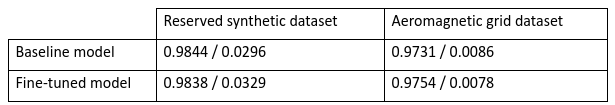
\includegraphics[width=\linewidth]{fig/p2/temp_tbl.png}
% % \begin{tblr}{ll}
% %                 & Reserved Synthetic Dataset & Reserved Aeromagnetic Dataset \\
% %                 & Mean / Standard Dev.       & Mean / Standard Dev.          \\
% %     \hline{}
% %     Baseline   & 0                          & 0                             \\
% %     Fine-Tuned & 0                          & 0                             \\
% % \end{tblr}
%     \caption[Accuracy Metrics]{Accuracy metrics for each upsampling method. The best performing method for each metric is bolded.}
%     \label{tab:2metrics}
% \end{table}


Qualitative results are shown to compare the outputs from the two models, the baseline model that is trained with synthetic data and the fine-tuned model trained with open access survey data.

\Cref{fig:srdata23,fig:srdata14,fig:srdata17,fig:srdata18} contain open access grid data from the Eastern Goldfields Superterrane of Western Australia, prepared using the proposed method.
Each figure follows the following layout for the grids; a) the ground truth (GT) \numproduct{200 x 200} cell tile is presented with low-resolution sampled data indicated in colour.
The target high-resolution grid (HR), created from sampling and gridding GT at \qty{80}{\m} line spacing, is shown in b) for comparison.
The \numproduct{45 x 45} cell low-resolution grid (LR) shows the result of the described sampling and gridding method at \qty{320}{m} line spacing, and is upscaled for display using bicubic interpolation in c).
The baseline model prediction (Baseline SR), using an input of LR with the proposed method, is shown in d) with the corresponding SSIM metric between HR and SR\@.
The fine-tuned model prediction is shown in e).

Strong line-perpendicular smearing in LR is reduced in both SR predictions, and fine structural divisions are better delineated.
NW striking features around in HR are aliased in LR and subsequently incorrectly rotated by 90 degrees in the baseline SR prediction (\Cref{fig:srdata23} d).
The fine-tuned model (\Cref{fig:srdata23} e) resolves the correct strike, and separates the two features present.
The enhanced structural similarity is reflected by the higher SSIM score in the fine-tuned model.

\begin{figure}[hbtp]
    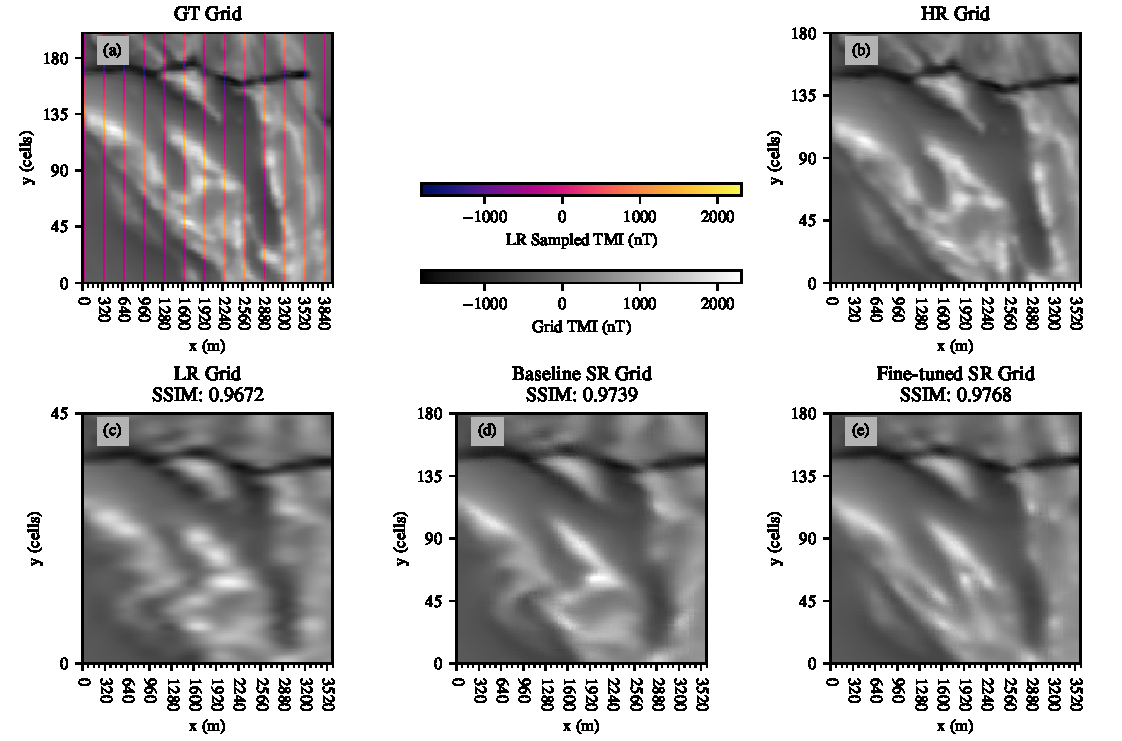
\includegraphics[width=0.9\linewidth]{fig/p2/srcomp_23.pdf}
    \caption[Super-resolution geophysics grid results]{Super-resolution predictions on open access data, prepared using the proposed method.
        Explanation in-text.
        Grid A is the super-resolution prediction using the baseline model, while grid B is the SR prediction using the fine-tuned model.}
    \label{fig:srdata23}
\end{figure}

\begin{figure}[hbtp]
    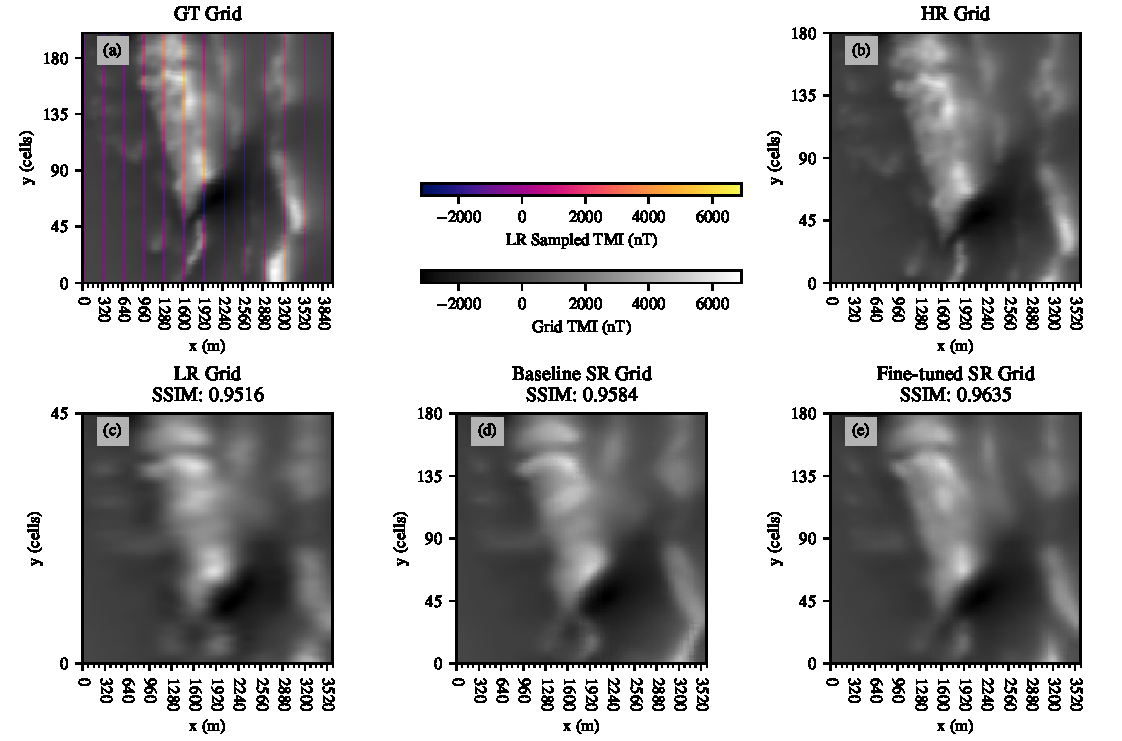
\includegraphics[width=0.9\linewidth]{fig/p2/srcomp_14.pdf}
    \caption[Super-resolution geophysics grid results]{Super-resolution predictions on open access data, prepared using the proposed method.
        Explanation in-text.
        Grid A is the super-resolution prediction using the baseline model, while grid B is the SR prediction using the fine-tuned model.}
    \label{fig:srdata14}
\end{figure}

\begin{figure}[hbtp]
    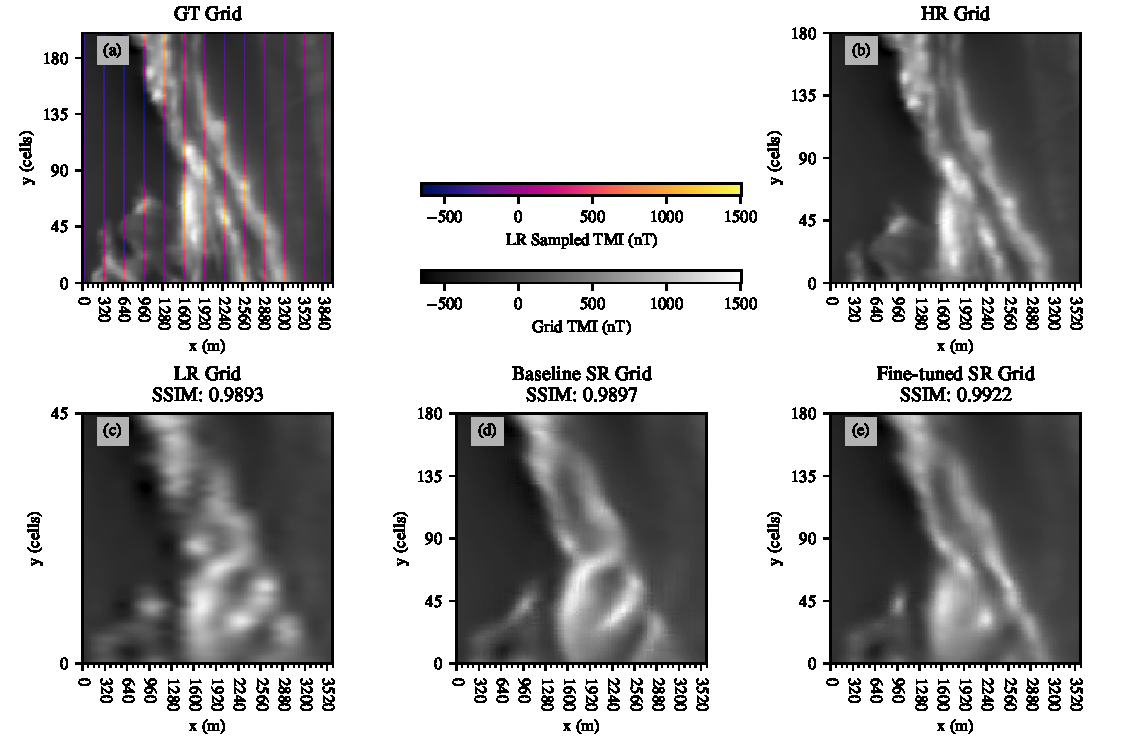
\includegraphics[width=0.9\linewidth]{fig/p2/srcomp_17.pdf}
    \caption[Super-resolution geophysics grid results]{Super-resolution predictions on open access data, prepared using the proposed method.
        Explanation in-text.
        Grid A is the super-resolution prediction using the baseline model, while grid B is the SR prediction using the fine-tuned model.}
    \label{fig:srdata17}
\end{figure}

\begin{figure}[hbtp]
    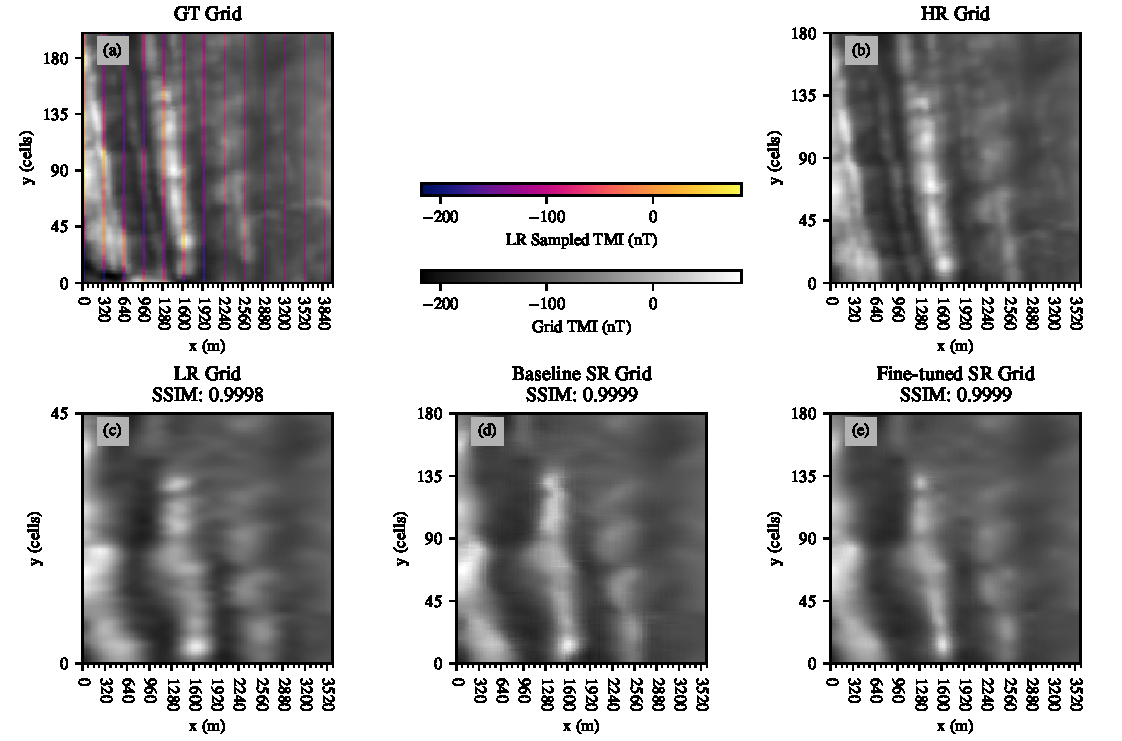
\includegraphics[width=0.9\linewidth]{fig/p2/srcomp_18.pdf}
    \caption[Super-resolution geophysics grid results]{Super-resolution predictions on open access data, prepared using the proposed method.
        Explanation in-text.
        Grid A is the super-resolution prediction using the baseline model, while grid B is the SR prediction using the fine-tuned model.}
    \label{fig:srdata18}
\end{figure}


\section{Discussion}
\label{sec:2discussion}
The Noddyverse synthetic training dataset comprises geology models with a variety of realistic petrophysics and geological histories, and was sampled using simple but realistic airborne survey methodology.
Furthermore, real survey data used to fine tune the model were extracted from extents across a range of different terranes in Western Australia.
As such, the method and trained models generalise to the geological terranes represented in the Noddyverse and high-resolution state grid extents.
Granitic textures in real grid data are not represented in the synthetic Noddyverse training set, and show the least improvement by the method.
Different geological units present different features in magnetic potential field grids, with deformed igneous units typically causing abundant contextually important short-wavelength content.
These features, such as faulted or folded dykes, tend to show the most perceptual improvement in their structure following super-resolution upscaling.
This is due to the high performance of the method for reducing aliasing effects from the gridding process, and is apparent in the accurate reconstruction of linear features from discrete “string of beads” aliased features.
Long-wavelength features and smooth gradients, such as those present in sedimentary units or areas of cover are accurately upscaled in the proposed method, however these are also adequately upscaled with simple cubic spline interpolation of the low-resolution grid because they do not require predicted high frequency components.
The exception for super-resolution having higher quality is in areas of low magnitude TMI of only a few nanotesla across the entire extent.
In these cases, the otherwise minor noise introduced by the super-resolution process dominates the residual.

The synthetic forward models are associated with geological history class labels, providing an opportunity for more targeted fine-tuning by event history.
It is possible to filter the data to contain only the events of interest, which would prepare a baseline model targeting a single geological domain.
The baseline model prepared in this work demonstrated good performance across a range of geological domains, but may be improved for targeted domains using the filtered approach.

\section{Conclusions}
\label{sec:2conclusion}
An approach for upscaling geologically diverse geophysical survey grid data is proposed, which adopts transfer learning from synthetic data to better generalise super-resolution across different geological domains.
Using the preeminent LTE neural network architecture, synthetic magnetic forward models were used to prepare a baseline model capable of upscaling survey grids at four times scale.
Further, this baseline model was fine-tuned with open access survey grid data, prepared with a low-resolution transform appropriate for aeromagnetic geophysics.
Low-resolution features incorrectly enhanced by the synthetic baseline model were correctly resolved following fine-tune training with these data, and the model is capable of upscaling grids with \qty{320}{\m} line spacing to \qty{80}{\m} line spacing with an average FSIM score of \num{0.9731}.

% \section{Declaration of Competing Interest}
% The authors declare the following financial interests / personal relationships which may be considered as potential competing interests: This work was supported by a Rio Tinto Iron Ore PhD scholarship.

\printbibliography{}


% \end{document}